\documentclass[twocolumn, 10pt]{article}

\usepackage[margin=1in]{geometry}
\usepackage[utf8]{inputenc}
\usepackage[T1]{fontenc}
\usepackage{hyperref}
\usepackage{url}
\usepackage{booktabs}
\usepackage{amsfonts}
\usepackage{nicefrac}
\usepackage{microtype}
\usepackage{graphicx}
\usepackage{amsmath}
\usepackage{authblk}
\usepackage{titlesec}

% Tighter spacing around section headings
\titlespacing*{\section}      {0pt}{1.4ex plus .3ex minus .2ex}{0.6ex plus .2ex}
\titlespacing*{\subsection}   {0pt}{1.0ex plus .3ex minus .2ex}{0.4ex plus .2ex}
\titlespacing*{\subsubsection}{0pt}{0.8ex plus .2ex minus .2ex}{0.3ex plus .2ex}
\titlespacing*{\paragraph}    {0pt}{0.6ex plus .2ex minus .1ex}{0.6em}

\graphicspath{{paper_figures/}{./paper_figures/}{../results/paper_figures/}}

\title{FinJEPA: Self-Supervised Market Regime Detection via Adaptive Joint Embeddings}

\author[1]{Ishan Malik}
\author[1]{Mehul Goel}
\author[1]{Sahil Parupudi}
\affil[1]{Center for Data Science, New York University\\
\texttt{\{im2854, mg8958, sp9019\}@nyu.edu}}

\date{}

\begin{document}

\maketitle

\begin{abstract}
  Identifying market regimes---Bear, Sideways, and Bull periods that
  govern return distributions---is central to quantitative finance, yet
  labels are unavailable and daily returns are dominated by noise. We
  introduce \textbf{FinJEPA}, the first Joint Embedding Predictive
  Architecture for financial time series. A Transformer context encoder,
  an EMA target encoder with a novel volatility-adaptive decay schedule,
  and a cross-attention predictor are trained to forecast
  \emph{representations} of held-out future S\&P~500 patches rather than
  raw returns, sidestepping the noise-overfitting trap of masked
  reconstruction. Under a frozen-encoder linear probe on HMM regime
  labels, FinJEPA more than doubles the macro-F1 of PatchTST and
  TS2Vec, with layer-wise probing showing abstract regimes emerging
  organically in deeper layers.
\end{abstract}

\section{Introduction \& Motivation}
% Define market regimes and their importance in quantitative finance.
% Challenge of unlabeled data and the need for SSL.
% Core thesis: predicting raw prices fails; latent prediction succeeds as a noise filter.
% Contributions: (1) JEPA in finance, (2) Adaptive EMA, (3) regime emergence.

\section{Related Work}
\label{sec:related}

FinJEPA draws on three lines of prior work: the classical literature on
market regime detection in quantitative finance, self-supervised learning
(SSL) for time series, and the more recent Joint Embedding Predictive
Architecture (JEPA) family. We summarise each in turn and then state how
FinJEPA differs.

\paragraph{Market regime detection.}
The textbook approach is the Hidden Markov Model
(HMM)~\cite{hamilton1989, ang2002, kim1999}: at any point in time the
market sits in one of $K$ hidden states, and the day's return is drawn
from a Gaussian whose mean and variance depend on the state. Given a
sequence of daily returns, the HMM produces one regime label per day via
the Viterbi algorithm~\cite{baum1970}. HMMs are interpretable, but they
assume returns are i.i.d.\ within a regime and that the number of regimes
is fixed in advance. More importantly for us, an HMM is a \emph{labeller},
not a representation learner---it outputs a discrete state per day, not a
feature vector that could be reused downstream. Because no public dataset
provides ground-truth regime labels for the S\&P~500, we follow common
practice~\cite{lopezdeprado2018, dixon2020} and treat the labels of a
3-state HMM, fit on the training period only, as our pseudo-ground-truth
reference. No representation-learning model in this paper sees these
labels during pretraining.

\paragraph{Self-supervised learning for time series.}
To learn representations without labels, the standard tool is SSL, and
two families dominate on time series. \emph{Contrastive} methods create
two augmented views of the same window and train an encoder to embed them
close together while pushing different windows apart; the canonical
time-series example is TS2Vec~\cite{yue2022ts2vec}, a dilated 1D~CNN
trained with a hierarchical contrastive loss, in the spirit of
SimCLR~\cite{chen2020simclr} and MoCo~\cite{he2020moco}. The other family
takes the opposite approach: rather than comparing two views, it hides
part of the input and asks the encoder to fill in what was hidden.
PatchTST~\cite{patchtst} is the strongest published example---it splits
the series into patches, masks some of them, and trains a Transformer to
reconstruct the missing raw values, following BERT~\cite{devlin2018bert}
and MAE~\cite{he2022mae}. Reconstruction works well when the input is
mostly signal, but daily financial returns are mostly noise, so the
encoder is forced to memorise that noise just to drive its loss down. We
therefore use TS2Vec and PatchTST as our two SSL baselines---one from each
family.

\paragraph{Joint embedding methods and JEPA.}
A third family avoids both contrastive negatives and raw-value
reconstruction by aligning two views directly in embedding space.
BYOL~\cite{grill2020byol}, SimSiam~\cite{chen2021simsiam}, and
DINO~\cite{caron2021dino} pair an ``online'' encoder updated by gradient
descent with a ``target'' encoder whose weights are an exponential moving
average (EMA) of the online one; the online network learns to predict
what the target produces, and the target itself receives no gradient.
Without negative samples the encoder could in principle collapse to a
constant, but methods such as VICReg~\cite{bardes2021vicreg} and Barlow
Twins~\cite{zbontar2021barlow} prevent this by regularising the variance
and covariance of the embeddings. JEPA~\cite{lecun2022path}, instantiated
for images by I-JEPA~\cite{ijepa} and for video by
V-JEPA~\cite{bardes2024vjepa}, ties these ideas together: a context
encoder reads part of the input, a small predictor maps its output into
the embedding space of the held-out part, and an EMA target encoder
produces what the predictor must match. The crucial design choice is that
the loss is computed on \emph{representations}, never on raw input, so
the encoder is not penalised for ignoring unpredictable details. JEPA has
been studied almost exclusively on images and video; financial time
series remain essentially unexplored.

\paragraph{Positioning of FinJEPA.}
FinJEPA adapts the JEPA recipe to financial markets, and differs from
each of the threads above in a specific way. Unlike an
HMM~\cite{hamilton1989}, it is a representation learner, not a
labeller---HMM labels enter our pipeline only at evaluation time, as the
target of a frozen-encoder linear probe. Unlike
TS2Vec~\cite{yue2022ts2vec}, it uses no augmentations and no negatives;
the pretext task is simply to predict the encoder's representation of the
next four months from the previous twelve. Unlike
PatchTST~\cite{patchtst}---with which we share patch size, hidden
dimension, and Transformer backbone exactly---the only thing we change
is what the model predicts (representations, not raw returns), so any
performance gap directly measures the effect of latent-vs.-input-space
prediction. Finally, unlike I-JEPA~\cite{ijepa}, we make two changes
specific to time series: the context/target split is \emph{causal} (the
past predicts the future, instead of filling in randomly hidden patches),
and the EMA decay rate $\tau$ is adjusted based on the realised batch
volatility, so the target encoder adapts faster during turbulent markets.

\section{Methodology}
\label{sec:methods}

\subsection{Data \& Preprocessing}
\label{sec:data}

\paragraph{Source.}
We use daily close prices of the S\&P~500 index (ticker \texttt{\^{}GSPC})
from 2000-01-01 to 2024-12-31, downloaded via Yahoo Finance, yielding
roughly 6{,}300 trading days that span the dot-com bust, the 2008
financial crisis, the 2020 COVID crash, and the 2022 bear market. We
choose the S\&P~500 because it is the most-studied index in the
regime-detection literature and because the 25-year window contains every
canonical regime type at least twice.

\paragraph{Log returns and causal normalisation.}
For each day $t$ we compute the log return $r_t = \log(P_t / P_{t-1})$.
Raw returns drift in mean and variance over decades, which would let the
encoder cheat by memorising the year. We therefore apply a strictly
\emph{causal} rolling z-score with a 252-day (one-trading-year) lookback,
\[
  \tilde{r}_t \;=\; \frac{r_t - \mu_t^{(252)}}{\sigma_t^{(252)}},
\]
so that the normalisation at time $t$ uses only information available at
time $t$. This eliminates lookahead leakage that plagues many published
financial benchmarks.

\paragraph{Patches and sliding windows.}
We tokenise the normalised return stream into non-overlapping
\emph{patches} of $P=20$ days ($\approx$ one trading month). Each training
example is a window of $C+T=12+4=16$ patches: the first $C=12$ patches
form the \textbf{context} and the last $T=4$ form the \textbf{target}.
We slide this window with stride $5$ (one trading week) to augment the
dataset roughly $4\times$ while keeping consecutive samples weakly
correlated.

\paragraph{Splits.}
We split chronologically: train = 2000--2017, validation = 2018--2020,
test = 2021--2024. The val period contains the COVID crash and the test
period contains the 2022 bear market, so probes are scored on regimes
genuinely unseen during pretraining.
Figure~\ref{fig:regime_timeline} shows the full normalised return stream
overlaid with regime labels.

\begin{figure*}[t]
  \centering
  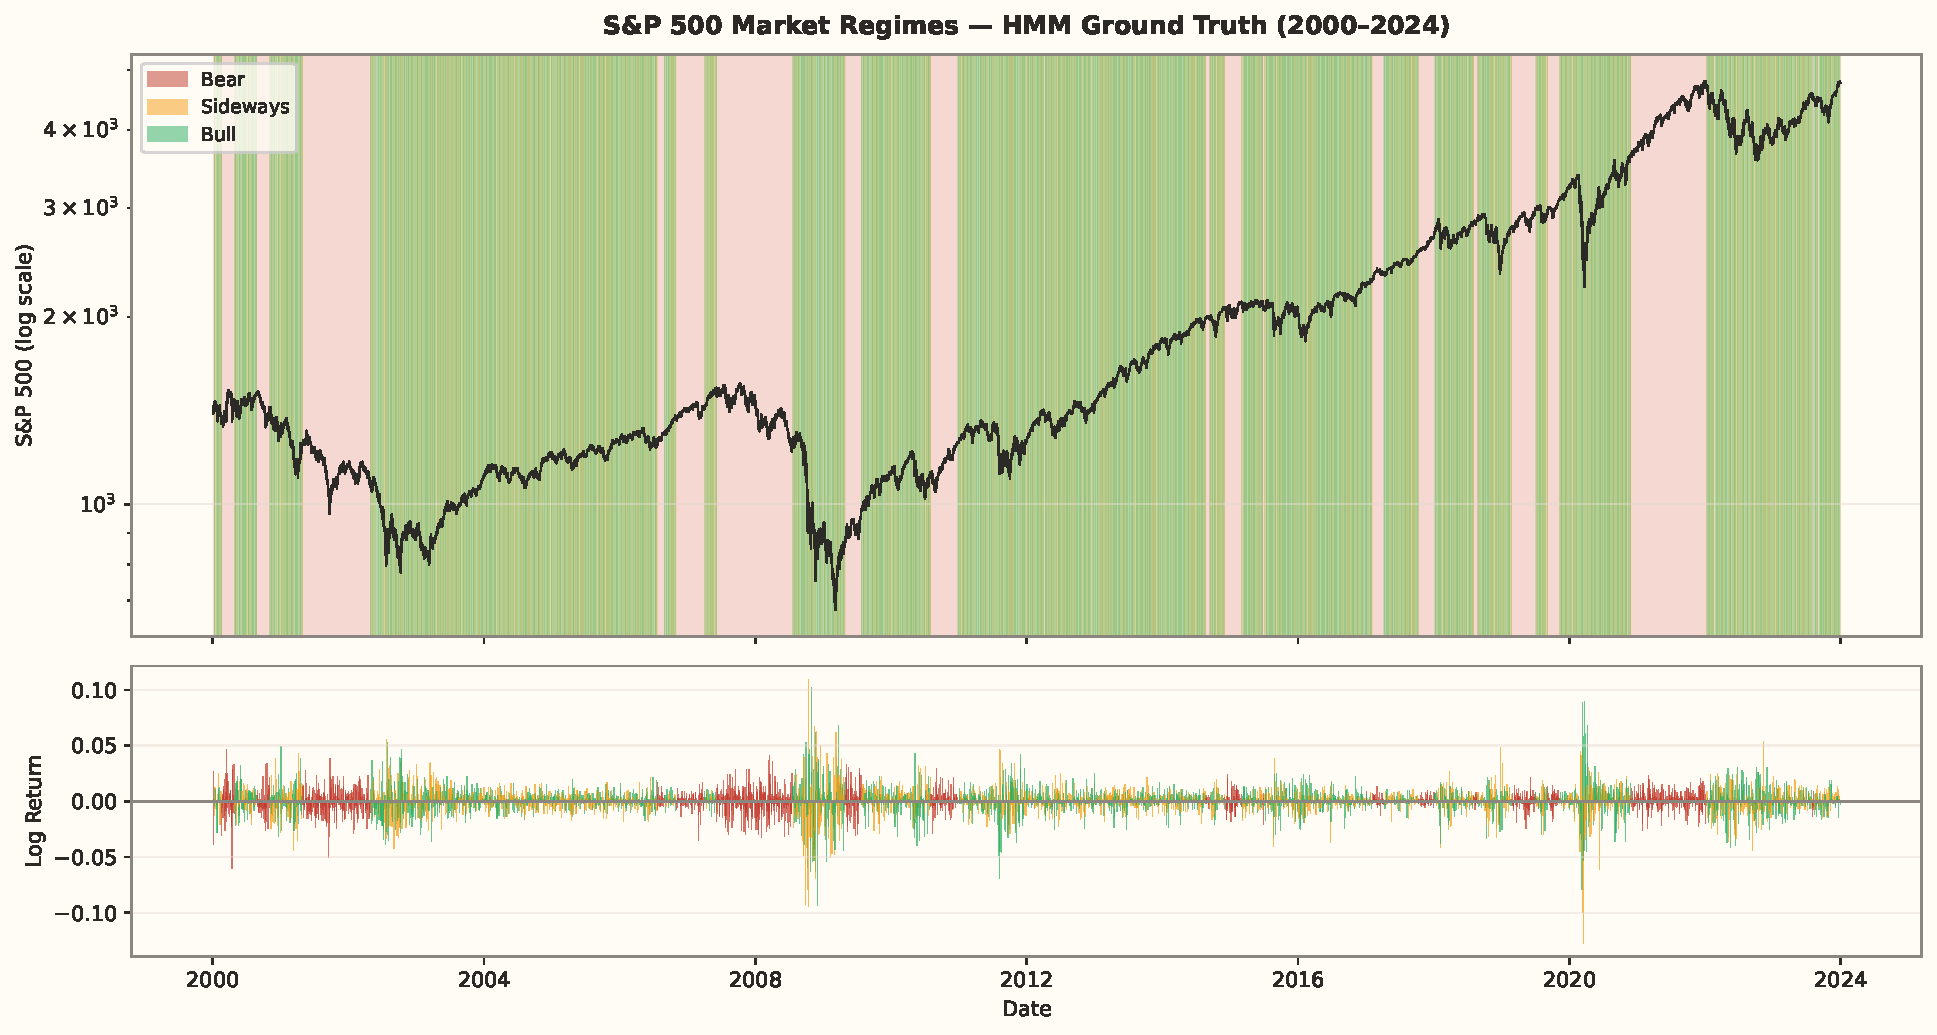
\includegraphics[width=0.95\textwidth]{fig01_regime_timeline.pdf}
  \caption{S\&P~500 normalised log returns (2000--2024) coloured by HMM
  regime. Vertical dashed lines mark the train/val/test split. The val
  and test periods include the 2020 COVID crash and the 2022 bear market.}
  \label{fig:regime_timeline}
\end{figure*}

\subsection{Ground-Truth Regime Labels}
\label{sec:hmm}

We obtain pseudo-ground-truth regime labels by fitting a 3-state Gaussian
HMM~\cite{hamilton1989, baum1970} to the training-period daily returns
\emph{only}; the HMM is then frozen and applied to val/test. The three
hidden states are sorted by their fitted mean return and labelled
\textbf{Bear} (0), \textbf{Sideways} (1), and \textbf{Bull} (2). We use
three states rather than two because real markets exhibit a distinct
low-volatility, near-zero-return regime that a Bull/Bear binary collapses
into noise.

\paragraph{Patch-level labels.}
Each 20-day patch receives a single label by majority vote of its 20 daily
labels. Patch labels are the targets of the linear probe used at
evaluation time; \emph{no} model in this paper sees these labels during
pretraining.

\paragraph{Class statistics.}
Table~\ref{tab:regime_stats} reports the per-state mean, volatility, and
transition probabilities; Figure~\ref{fig:regime_distribution} shows the
patch-level class distribution. Bull dominates by sample count, while
Bear is the rarest and most volatile state---the class for which Macro-F1
matters most.

\begin{table}[t]
\centering
\small
\caption{HMM Regime Statistics — S\&P~500 (2000--2024). Returns are daily log returns. Annualised figures assume 252 trading days.}
\label{tab:regime_stats}
\begin{tabular}{lcccc}
\toprule
Regime & Days (\%) & Ann.\ Mean (\%) & Ann.\ Vol (\%) & Skewness \\
\midrule
  Bear & 1867 (30.9\%) & +3.22 & 19.54 & -0.151 \\
  Sideways & 519 (8.6\%) & -12.24 & 21.26 & 0.074 \\
  Bull & 3650 (60.5\%) & +8.29 & 19.46 & -0.574 \\
\bottomrule
\end{tabular}
\end{table}

\begin{figure}[t]
  \centering
  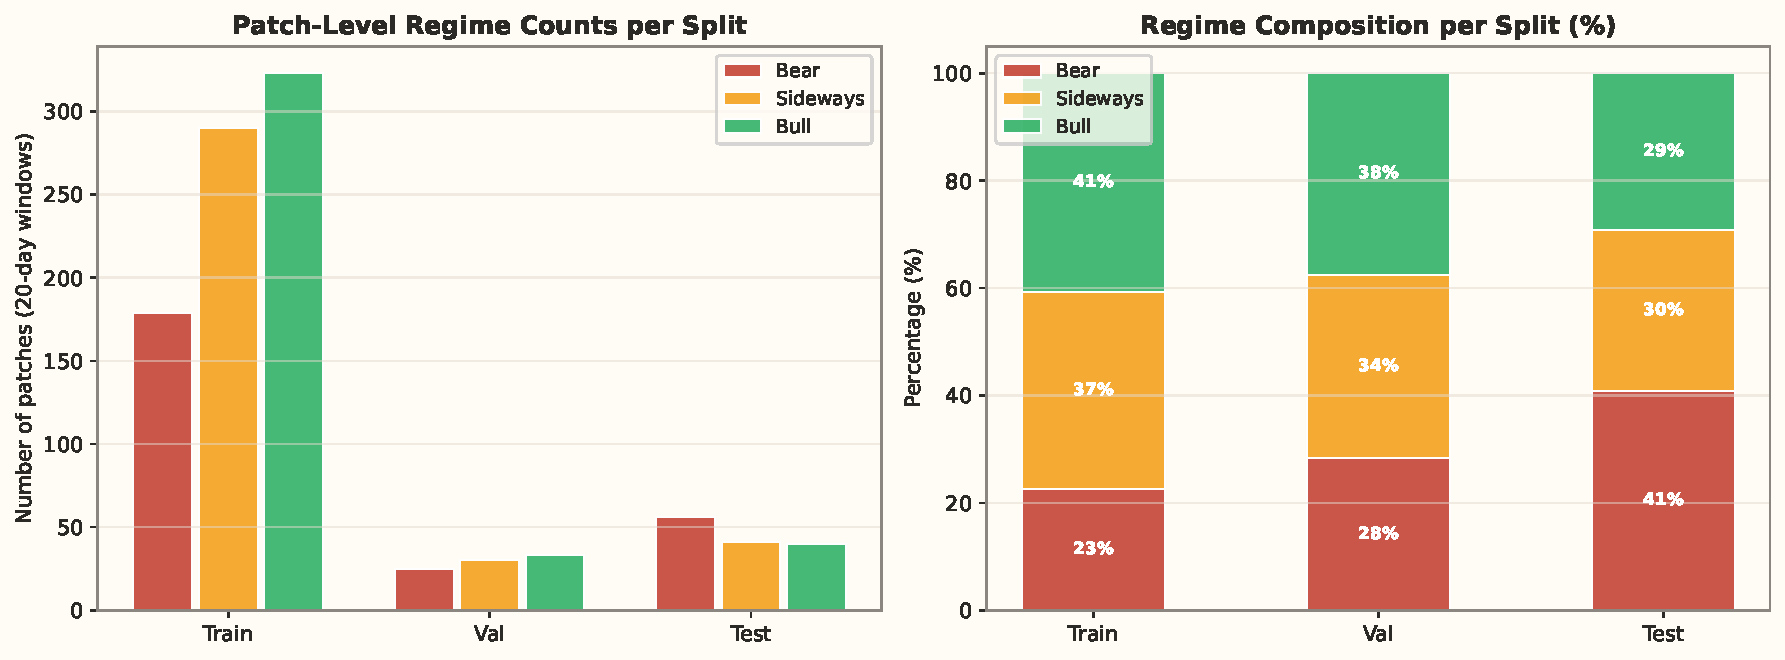
\includegraphics[width=\linewidth]{fig02_regime_distribution.pdf}
  \caption{Patch-level distribution of HMM regime labels in the train,
  validation, and test splits. Bear is the minority class in every split,
  motivating Macro-F1 over plain accuracy.}
  \label{fig:regime_distribution}
\end{figure}

\subsection{FinJEPA Architecture}
\label{sec:finjepa}

FinJEPA has three components: a \textbf{context encoder} $f_\theta$, a
\textbf{target encoder} $f_\xi$, and a \textbf{predictor} $g_\phi$.

\paragraph{Patch embedding.}
Each patch $x_i \in \mathbb{R}^{20}$ is linearly projected to a
$d=384$-dimensional token, summed with a learnable positional embedding,
and layer-normalised.

\paragraph{Encoders.}
Both $f_\theta$ and $f_\xi$ are 6-layer pre-norm Transformers with $h=6$
attention heads and feed-forward dimension $4d$. The context encoder
$f_\theta$ is updated by the optimiser; the target encoder $f_\xi$ is
\emph{not}. Instead, $f_\xi$ is initialised as an exact copy of
$f_\theta$ and updated as an exponential moving average (EMA),
\[
  \xi \;\leftarrow\; \tau\,\xi + (1-\tau)\,\theta,
\]
with $\theta$ kept under a stop-gradient when computing the target. This
is the standard BYOL/I-JEPA recipe~\cite{grill2020byol, ijepa}.

\paragraph{Predictor.}
The predictor $g_\phi$ is a single cross-attention block. It owns $T=4$
learnable target-position queries which attend to the context
representations $f_\theta(x_{1:C})$ as keys/values. The output is a
sequence of predicted target representations
$\hat{z}_{C+1:C+T} \in \mathbb{R}^{T \times d}$.

\paragraph{Training objective.}
The training loss is a Smooth-L1 regression in representation space,
\[
  \begin{aligned}
    \mathcal{L}_{\text{JEPA}} \;=\; \mathrm{SmoothL1}\big(\;
      & g_\phi(f_\theta(x_{1:C})), \\[-2pt]
      & \mathrm{sg}(f_\xi(x_{C+1:C+T}))\;\big),
  \end{aligned}
\]
where $\mathrm{sg}(\cdot)$ is stop-gradient. To prevent representational
collapse without negatives we add a VICReg-style variance
penalty~\cite{bardes2021vicreg},
$\mathcal{L}_{\text{var}} = \mathbb{E}\big[\,\mathrm{ReLU}(1 -
\sigma_d(z))\,\big]$, computed over the per-dimension standard deviation
of the context outputs. The full loss is
$\mathcal{L} = \mathcal{L}_{\text{JEPA}} + 5\,\mathcal{L}_{\text{var}}$.

\subsection{Adaptive EMA Schedule}
\label{sec:adaptive-ema}

A fixed $\tau$ assumes the target encoder should evolve at a constant
rate, which is poorly suited to financial data: in calm markets the
target should be stable, but in volatile periods (e.g.\ March 2020)
holding the target fixed anchors the predictor to a stale, pre-crash
representation. We therefore make $\tau$ a function of the realised
batch volatility $v$ (the standard deviation of z-scored returns in the
batch),
\[
  \tau(v) \;=\; \tau_{\max} - (\tau_{\max} - \tau_{\min})\,
                 \tanh(\lambda\,v),
\]
with $\tau_{\min}=0.990$, $\tau_{\max}=0.999$, and $\lambda=1.5$.
High-volatility batches receive a lower $\tau$, so the target encoder
adapts faster. The schedule is monotone, bounded, and adds zero
trainable parameters; it preserves the JEPA collapse-avoidance
properties of a slow EMA target while letting the target track regime
shifts when they happen.

\section{Experimental Setup \& Evaluation Protocol}
\label{sec:setup}

\subsection{Baselines \& The Probing Protocol}
% Supervised, TS2Vec, PatchTST. Frozen encoder + linear probe on HMM labels.

\subsection{Metrics Justification}
% Macro-F1 (class imbalance), Silhouette (cluster quality), per-class F1.

\section{Results \& Discussion}
\label{sec:results}

\subsection{Overall Representation Quality}
% Table 1 + UMAP discussion.

\subsection{Tracking Regime Emergence (Layer-Wise Analysis)}
% Layer-wise F1 — physical proof of the noise-filter thesis.

\subsection{Robustness and Statistical Significance}
% Bootstrap CIs.

\section{Conclusion \& Future Work}
% Summary; latent-space SSL wins on noisy financial data.
% Adaptive EMA helps in volatile regimes.
% Future: downstream RL on FinJEPA embeddings.

\begin{thebibliography}{99}

\bibitem{hamilton1989}
James D. Hamilton.
\newblock A new approach to the economic analysis of nonstationary time series and the business cycle.
\newblock \emph{Econometrica}, 57(2):357--384, 1989.

\bibitem{ang2002}
Andrew Ang and Geert Bekaert.
\newblock International asset allocation with regime shifts.
\newblock \emph{The Review of Financial Studies}, 15(4):1137--1187, 2002.

\bibitem{kim1999}
Chang-Jin Kim and Charles R. Nelson.
\newblock \emph{State-Space Models with Regime Switching}.
\newblock MIT Press, 1999.

\bibitem{baum1970}
Leonard E. Baum, Ted Petrie, George Soules, and Norman Weiss.
\newblock A maximization technique occurring in the statistical analysis of probabilistic functions of Markov chains.
\newblock \emph{Annals of Mathematical Statistics}, 41(1):164--171, 1970.

\bibitem{lopezdeprado2018}
Marcos L\'{o}pez de Prado.
\newblock \emph{Advances in Financial Machine Learning}.
\newblock Wiley, 2018.

\bibitem{dixon2020}
Matthew F. Dixon, Igor Halperin, and Paul Bilokon.
\newblock \emph{Machine Learning in Finance: From Theory to Practice}.
\newblock Springer, 2020.

\bibitem{lecun2022path}
Yann LeCun.
\newblock A path towards autonomous machine intelligence.
\newblock OpenReview, 2022.

\bibitem{ijepa}
Mahmoud Assran et al.
\newblock Self-supervised learning from images with a joint-embedding predictive architecture.
\newblock In \emph{CVPR}, 2023.

\bibitem{bardes2024vjepa}
Adrien Bardes et al.
\newblock V-JEPA: Latent video prediction for visual representation learning.
\newblock \emph{arXiv:2404.08471}, 2024.

\bibitem{grill2020byol}
Jean-Bastien Grill et al.
\newblock Bootstrap your own latent.
\newblock In \emph{NeurIPS}, 2020.

\bibitem{caron2021dino}
Mathilde Caron et al.
\newblock Emerging properties in self-supervised vision transformers.
\newblock In \emph{ICCV}, 2021.

\bibitem{chen2021simsiam}
Xinlei Chen and Kaiming He.
\newblock Exploring simple Siamese representation learning.
\newblock In \emph{CVPR}, 2021.

\bibitem{he2020moco}
Kaiming He et al.
\newblock Momentum contrast for unsupervised visual representation learning.
\newblock In \emph{CVPR}, 2020.

\bibitem{chen2020simclr}
Ting Chen et al.
\newblock A simple framework for contrastive learning of visual representations.
\newblock In \emph{ICML}, 2020.

\bibitem{bardes2021vicreg}
Adrien Bardes, Jean Ponce, and Yann LeCun.
\newblock VICReg: Variance-invariance-covariance regularization for self-supervised learning.
\newblock In \emph{ICLR}, 2022.

\bibitem{zbontar2021barlow}
Jure Zbontar et al.
\newblock Barlow Twins: Self-supervised learning via redundancy reduction.
\newblock In \emph{ICML}, 2021.

\bibitem{patchtst}
Yuqi Nie, Nam H. Nguyen, Phanwadee Sinthong, and Jayant Kalagnanam.
\newblock A time series is worth 64 words: Long-term forecasting with transformers.
\newblock In \emph{ICLR}, 2023.

\bibitem{yue2022ts2vec}
Zhihan Yue et al.
\newblock TS2Vec: Towards universal representation of time series.
\newblock In \emph{AAAI}, 2022.

\bibitem{dosovitskiy2020vit}
Alexey Dosovitskiy et al.
\newblock An image is worth 16x16 words: Transformers for image recognition at scale.
\newblock In \emph{ICLR}, 2021.

\bibitem{devlin2018bert}
Jacob Devlin et al.
\newblock BERT: Pre-training of deep bidirectional transformers for language understanding.
\newblock In \emph{NAACL}, 2019.

\bibitem{he2022mae}
Kaiming He et al.
\newblock Masked autoencoders are scalable vision learners.
\newblock In \emph{CVPR}, 2022.

\end{thebibliography}

\end{document}
